\section{Huge Pages}
	\label{sec:hugepage}
Huge pages are an optimization for performance. On latest Intel x86-64
platform, the page size can be even 1GB. This provides good chance for
applications to tune their performance, like the databases, or the host mode
virtual machine monitors. The benefits of huge pages have been long mentioned,
but viewing from the virtual memory system, it can be cost, like to prepare
these huge pages will rearrange memory so it is physical continuous. Moreover,
when page fault happens, it's much heavier than small page faults. In this
section, I try to show the cost of huge pages.

\subsection{Methodology}
The experiments focuses on the cost of allocating huge pages. Preparation time
can be quite long, but it is a one time cost, and will be much less possible to
become a bottleneck. So I will care more about what happened during using the
huge pages. What I did was allocating same amount of memory using both large
and small pages, and comparing the time elapsed with both sequential walking,
and random accessing. Also, I will increase the walking iteration, so that I
can find out what frequency of use can make huge pages competitive in
performance , even it has much larger overhead to be set up and zeroed out.

\subsection{Experiments}

\begin{figure}[hbt]
\centering
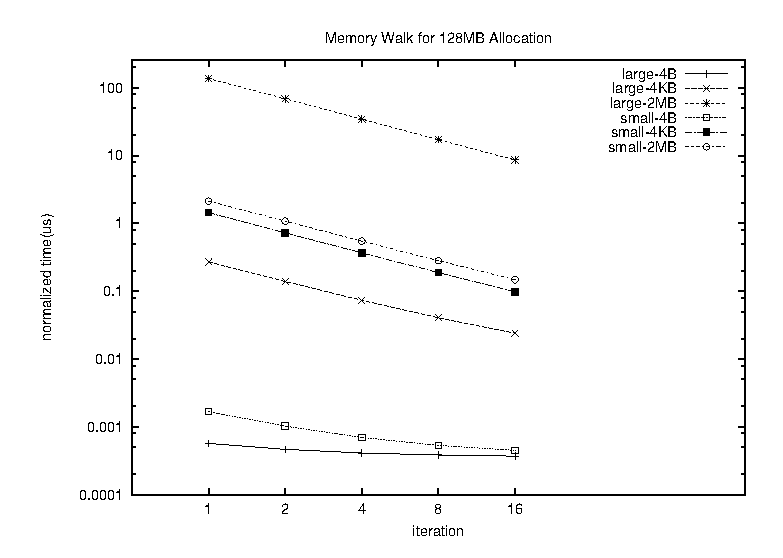
\includegraphics[width=0.9\linewidth]{../figures/hugetlb_128m}
\caption{Memory walk time on 128MB mapped memory. I use different stride, and
iterations for each walk, and measure the average time cost. The larger the 
stride size is, the worse performance I will get by using huge pages. Due to
space limitation, I didn't draw more stride result. Actually the small page
start to beat huge ones from the point of 32KB stride.}
\label{fig:hugetlb-time}
\end{figure}
\begin{figure}[h]
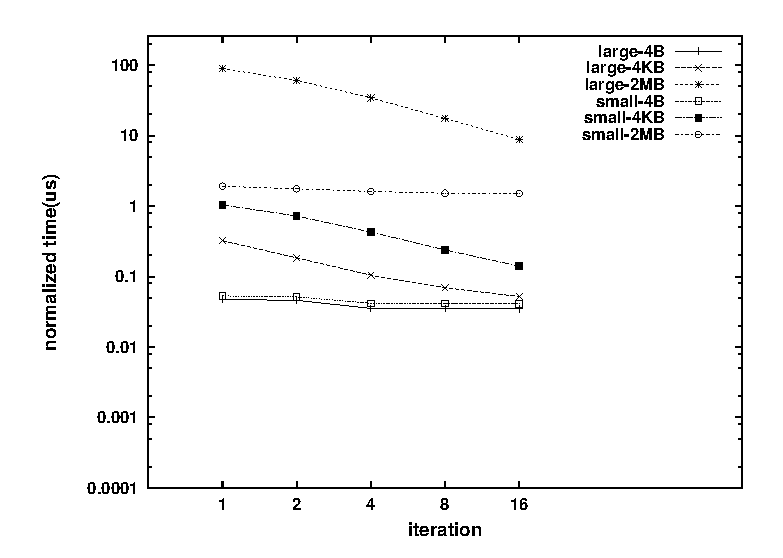
\includegraphics[width=0.9\linewidth]{../figures/hugetlb_rand_128m}
\caption{Random walking is similar with sequential walking, when in small stride
size the huge pages perform better. Here the stride is just used to determine
the amount of memory reference, rather than walk pattern. I use stride to label
it for comparison with sequential walk. One thing changes in random walk is
that for 4B stride, both of the two configurations perform worse than
sequential walk. The reason may be related with locality, but it is not what we
address here.}
\label{fig:hugetlb-rand}
\end{figure}

Figure~\ref{fig:hugetlb-time} shows the cost of walking on newly allocated
small and huge pages, total memory size is 128MB. The stride we used to walk on
the pages are from 4B to 2MB, with multiple iterations in each walk. It is quite
clear that huge pages performs bad when iteration number is small, and stride
is large. With the iteration increasing, its average performance becomes better.

Random walking shows similar trend as in figure~\ref{fig:hugetlb-rand}. Small
pages still perform better at the beginning, but normalized difference is
smaller. The result again illustrates the benefit of on demand allocation:
setting up the mapping and zeroing out pages at the very beginning is not a must, since the applications may not reference them all.

\subsection{Discussion}
Although there are some inconveniences, huge pages are useful, especially
when used by VMM. If no huge pages are used, then on a 4 level paging system, a
page fault can require up to 20 times memory reference. With the huge pages,
this can be reduced to minimum. The problem for the huge page is that it must
be configured and requested explicitly, thus may lead to memory pressure.
Another thing is the recognition of the cost of huge pages: for large data not
frequently referenced, using large pages may not get benefits.

During experimentation, I found a strange thing:in Linux normal users can get
huge page through \emph{mmap} interface using anonymous mapping, without
causing protection errors. However, the similar access through \emph{shmget}
interface will not work, unless super user privilege is granted. I didn't see
any differences between these two approaches, hopefully it is not a security hole.
